% Figure 1.6 — Retrieval / reader path decisions (Path A vs B, budget)
\documentclass[tikz,border=10pt]{standalone}
% Shared preamble for DARS journal figures (input from each fig_*.tex in this directory).
\usepackage[T1]{fontenc}
\usepackage{microtype}
\usepackage{helvet}
\renewcommand{\familydefault}{\sfdefault}
\usepackage{amssymb}
\usepackage{amsmath}
\usepackage{xcolor}
% tikz loaded by standalone class option [tikz]
\usetikzlibrary{positioning,arrows.meta,calc,fit,backgrounds,shapes.geometric,matrix}
\usepackage{pgfplots}
\pgfplotsset{compat=1.18}
\usepackage{pgfplotstable}
\usepackage{booktabs}
\usepackage{array}

% Print-safe palette (grayscale + one accent)
\definecolor{DarsAccent}{HTML}{2E5AAC}
\definecolor{DarsAccentDark}{HTML}{1A3D6E}
\definecolor{DarsGray}{HTML}{555555}
\definecolor{DarsLight}{HTML}{E8EBF0}
\definecolor{DarsBand}{HTML}{F4F5F7}

\tikzset{
  darsLine/.style={-{Stealth[length=2.2mm]}, line width=0.55pt, draw=DarsGray},
  darsLineAccent/.style={-{Stealth[length=2.2mm]}, line width=0.65pt, draw=DarsAccent},
  darsDash/.style={dashed, line width=0.5pt, draw=DarsGray!70},
  box/.style={draw=DarsGray, rounded corners=2.5pt, line width=0.5pt,
    fill=white, align=center, inner sep=4pt, font=\footnotesize\sffamily},
  boxFill/.style={box, fill=DarsLight},
  boxAccent/.style={box, draw=DarsAccent, line width=0.6pt, fill=DarsLight!60!white},
  lbl/.style={font=\scriptsize\sffamily, text=DarsGray},
  subnote/.style={font=\scriptsize\sffamily, text=DarsGray, align=left, anchor=north west},
  bigLbl/.style={font=\small\bfseries\sffamily, text=DarsAccentDark},
}

\begin{document}
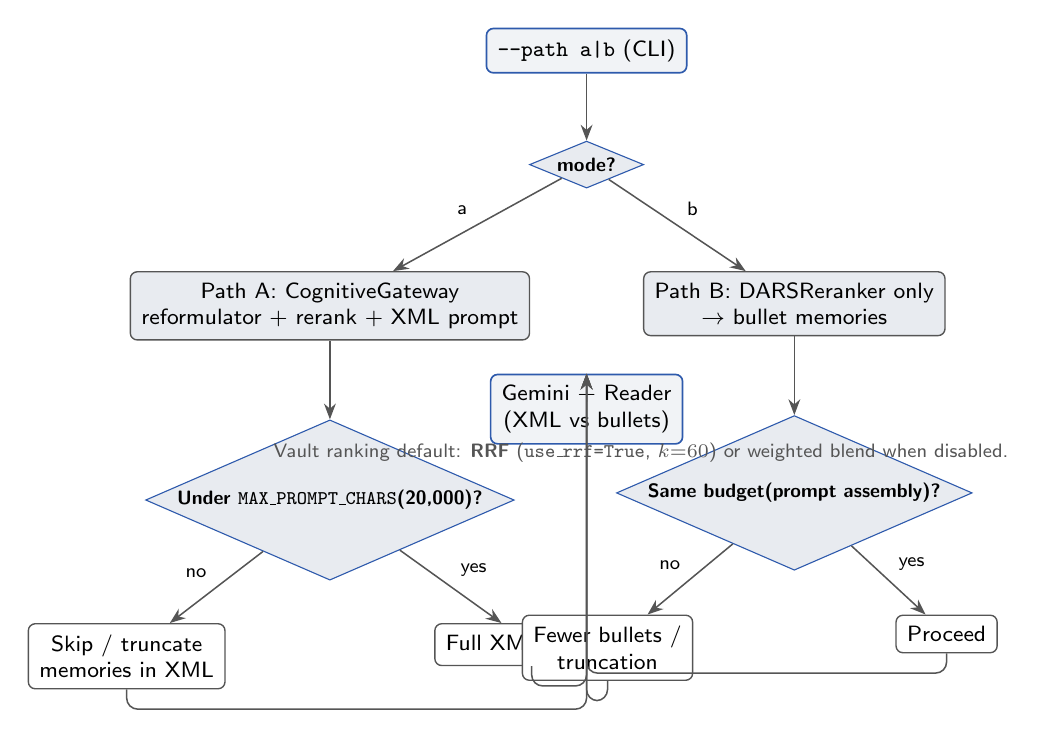
\begin{tikzpicture}[
  font=\footnotesize\sffamily,
  arr/.style={-{Stealth[length=2mm]}, line width=0.55pt, draw=DarsGray},
  dec/.style={diamond, aspect=2.3, draw=DarsAccent, fill=DarsLight, inner sep=1pt,
    font=\scriptsize\bfseries, minimum width=1.45cm},
]

  \node[boxAccent] (cli) at (0,0) {\texttt{--path a|b} (CLI)};
  \node[dec, below=0.85 of cli] (which) {mode?};
  \node[boxFill, below left=1.2 and 0.35 of which] (pa) {Path A: CognitiveGateway\\reformulator + rerank + XML prompt};
  \node[boxFill, below right=1.2 and 0.35 of which] (pb) {Path B: DARSReranker only\\$\rightarrow$ bullet memories};
  \node[dec, below=1.0 of pa] (truncA) {Under \texttt{MAX\_PROMPT\_CHARS}\\(20{,}000)?};
  \node[dec, below=1.0 of pb] (truncB) {Same budget\\(prompt assembly)?};
  \node[box, below left=1.05 and 0.15 of truncA] (dropA) {Skip / truncate\\memories in XML};
  \node[box, below right=1.05 and 0.15 of truncA] (okA) {Full XML prompt};
  \node[box, below left=1.05 and 0.15 of truncB] (dropB) {Fewer bullets /\\truncation};
  \node[box, below right=1.05 and 0.15 of truncB] (okB) {Proceed};
  \node[boxAccent, below=2.35 of which] (gem) {Gemini + Reader\\(XML vs bullets)};
  \draw[arr] (cli) -- (which);
  \draw[arr] (which) -- node[above left, font=\scriptsize] {a} (pa);
  \draw[arr] (which) -- node[above right, font=\scriptsize] {b} (pb);
  \draw[arr] (pa) -- (truncA); \draw[arr] (pb) -- (truncB);
  \draw[arr] (truncA) -- node[above left, font=\scriptsize] {no} (dropA);
  \draw[arr] (truncA) -- node[above right, font=\scriptsize] {yes} (okA);
  \draw[arr] (truncB) -- node[above left, font=\scriptsize] {no} (dropB);
  \draw[arr] (truncB) -- node[above right, font=\scriptsize] {yes} (okB);
  \draw[arr, rounded corners] (okA.south) -- ++(0,-0.25) -| (gem.north);
  \draw[arr, rounded corners] (dropA.south) -- ++(0,-0.25) -| (gem.north);
  \draw[arr, rounded corners] (okB.south) -- ++(0,-0.25) -| (gem.north);
  \draw[arr, rounded corners] (dropB.south) -- ++(0,-0.25) -| (gem.north);

  \node[subnote, anchor=west] at (-4.1,-5.1) {Vault ranking default: \textbf{RRF} (\texttt{use\_rrf=True}, $k{=}60$) or weighted blend when disabled.};

\end{tikzpicture}
\end{document}
